\documentclass{article}
\usepackage[utf8]{inputenc}
\usepackage[margin=0.70in]{geometry}
\usepackage{hyperref}
\usepackage{graphicx}
\usepackage{authblk}
\usepackage{subfig}

\title{Project 1: DNN Pruning via NNI}
\author{Oliver Fowler}
\author{Brian Park}
\affil{North Carolina State University, Computer Science 591/791-025}
\date{October 2022}

\begin{document}

\maketitle

\section{Pruning Methods}
%(1) What pruning methods you have applied to which DNN model.
For this project, we applied pruning models to a simple CNN and a state of the art ResNet model \cite{resnet}. To warm up, we used a simple \verb|L1NormPruner| \cite{l1prune} from NNI \cite{nni} to quickly get familiar with the workflow on a simple CNN provided by PyTorch. We performed this dataset on the MNIST digit dataset, which is a relatively easy dataset to train on for the purposes of quick development and experimental results.

Then we stepped it up a notch and used ResNet-101 to train the weights using the CIFAR-10 dataset, a much more complex dataset than MNIST. We used torchvision's collection of premade models rather than writing the model from scratch \cite{torchvision}. This took longer to train (180 epochs), but we wanted to see the magnitude of effect that structured pruning can have on a very deep neural network. For this network, we tried evaluated three different pruners: \verb|LevelPruner|, \verb|L1NormPruner|, \verb|L2NormPruner| \cite{levelpruner, l1prune}. But we still found \verb|L1NormPruner| to be the best performing in terms of accuracy and performance tradeoffs.

\section{Pruning and Hardware Configurations}
%(2) What configurations did you try on each pruning method, and what machine(s) you have used, including the CPU and GPU models of the machine(s).

\subsection{Hardware Configuration}
For hardware configurations, we fortunately had many devices with different architectures available to us. Not only on the ARC Cluster \cite{arc} do we have multiple GPUs, but we were also able to experiment on Brian's M1 MacBook Pro. Brian's M1 MacBook Pro features a 10-Core CPU with 8 performance cores and 2 efficiency cores, and 16-Core GPU with 32GB of unified memory. It also features a 16-core Neural Engine \cite{m1}. PyTorch recently announced native M1 support via Apple's Metal Performance Shaders \cite{pytorchm1}. It's able to perform operations like convolutional kernels optimally on the M1 GPU. Oliver used an Nvidia RTX 3080 on his local desktop computer.

For ARC, we used the NVIDIA A100 GPU \cite{a100}. It has 80GB of HBM and it claims 19.5 TFLOPS of FP32 performance. Fortunately, PyTorch enables CUDA specific features some by default, and others by some flags. We were also able to use NVIDIA's custom floating point format, TensorFloat32, as well as use 16 bit floating point numbers which the PyTorch API was aware of.


\subsection{Pruning Configuration}
For the pruning configurations, we used \verb|L1NormPruner| on the simple MNIST CNN as outlined by the NNI QuickStart Guide. We retrained for 3 more epochs after the pruning step. We tried pruning \verb|Conv2d| and \verb|Linear| leaving the last layer excluded for pruning. We experimented with \verb|L1NormPruner| and \verb|L2NormPruner|, but found \verb|L1NormPruner| the best in terms of accuracy.

For the second model, we chose ResNet-101, which is a much deeper DNN. We wanted to see the effects that residual connections have on deep neural networks. We used the CIFAR-10 dataset as that's a relatively more challenging dataset than MNIST. As for which pruner we used, we brute forced the search for the best pruning method. Training multiple pruning methods on the same dataset is an embarrassingly parallel problem, so we used Ray to exploit this parallelism on the A100 GPU \cite{ray}. Ray is a distributed framework for scaling AI and Python applications. Since there is no communication between the training processes, we really could've used any other distributed programming framework. But we chose Ray as it has GPU support, and it's able to support multi process Python execution on a single GPU. We see that once we train in parallel, we can fully utilize the memory usage as well as the GPU utilization as shown in the output of \verb|nvidia-smi| in Figure \ref{fig:nvidiasmi}. We retrained for 20 more epochs after the pruning step, since this is a much deeper network. We experimented with \verb|LevelPruner|, \verb|L1NormPruner|, \verb|L2NormPruner|. We found that pruning with only \verb|Conv2d| and excluding the last layer showed the best results.

For both networks, we pruned from 10\% to 90\% sparsity ratios with intervals of 10\%. We experimented with pruners such as \verb|LevelPruner|, \verb|L1NormPruner|, \verb|L2NormPruner| \cite{levelpruner, l1prune}.


\begin{figure}
	\centerline{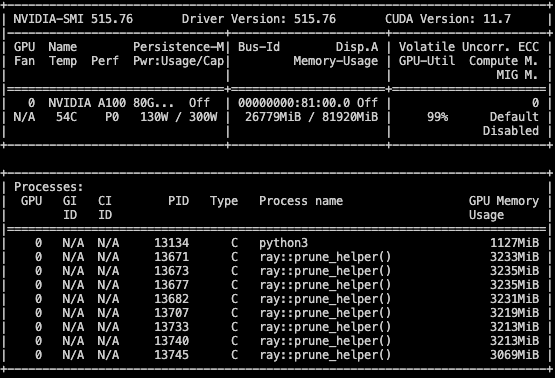
\includegraphics[width=6in]{../proj1/figures/nvidia-smi_pruning.png}}
	\caption{Peak GPU utilization}
	\label{fig:nvidiasmi}
\end{figure}

\section{Experimental Results}
%(3) What results you have obtained, including the output of "print(model)" of your original model and pruned model, their running speeds and accuracies;

\begin{figure}
	\centerline{
		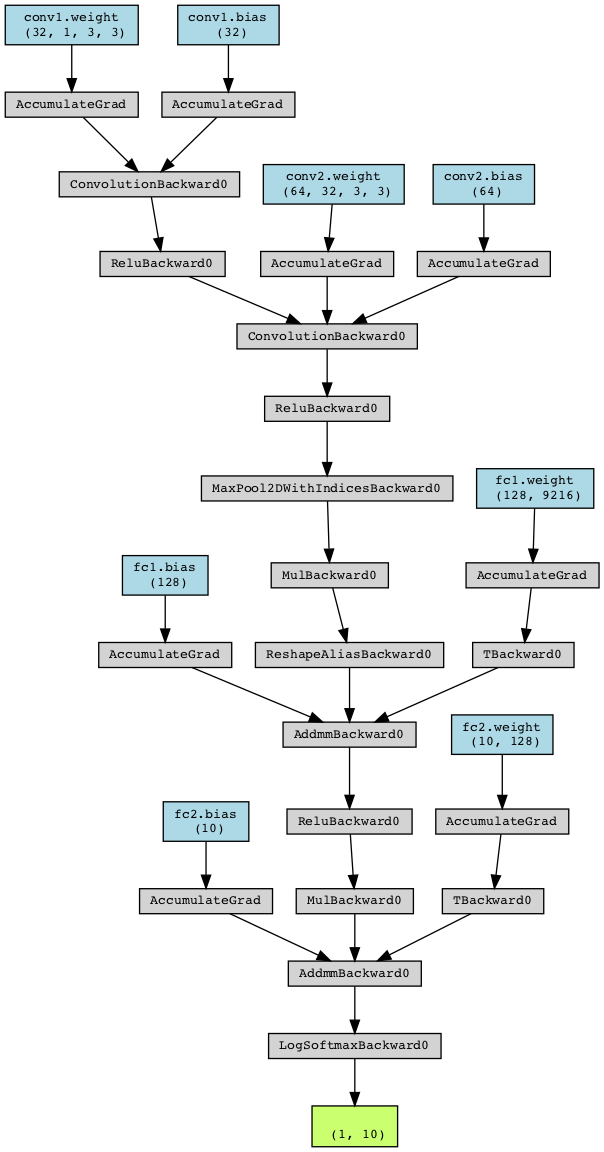
\includegraphics[width=2in]{../proj1/figures/mnist_cnn.png}
		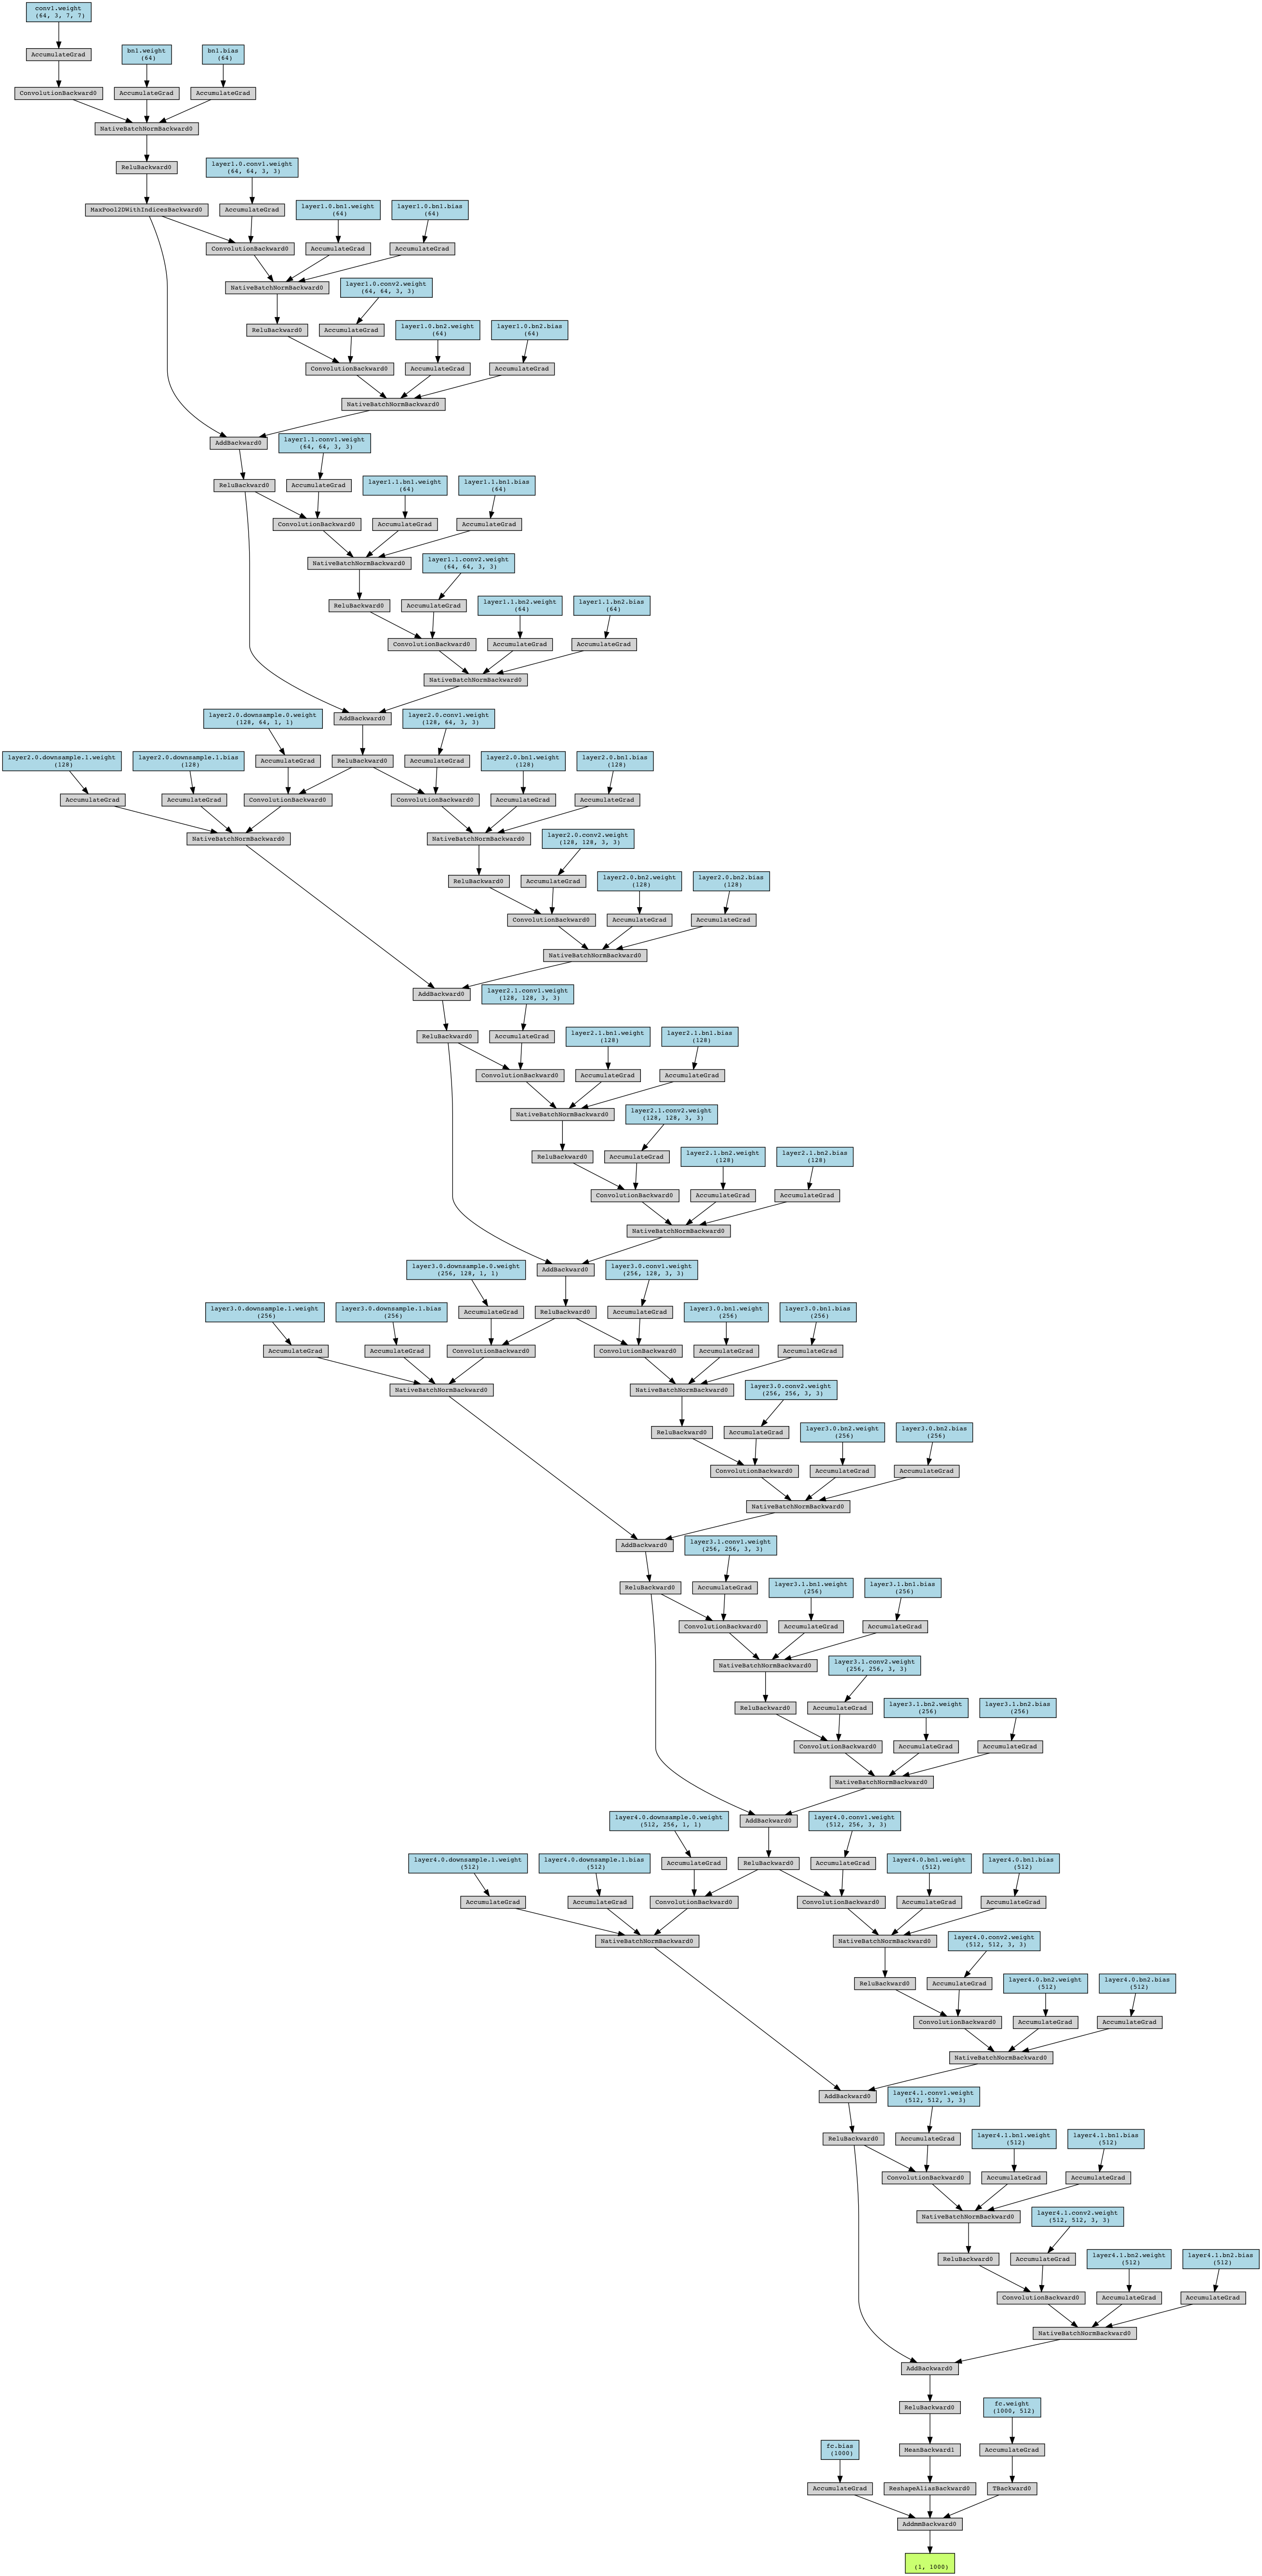
\includegraphics[width=2in]{../proj1/figures/resnet18.png}
	}
	\caption{DNN Computation Graphs}
	\label{fig:dnngraph}
\end{figure}

The outputs of \verb|print(model)| is shown for \hyperref[sec:A1]{Simple CNN} and \hyperref[sec:A2]{ResNet-18} in Appendix A. For visuals, we outputted the graph of the DNNs as well in Figure \ref{fig:dnngraph}. Note that although we used ResNet-101 for the report, the print output and computation graph are showing ResNet-18 for readability. For the Simple CNN, we show both the outputs before and after pruning.

After training each model, we benchmarked both models for their inference time as a baseline. Then we used NNI to prune as aggressively as we could to showcase the performance vs. accuracy degradation trade-off. Unfortunately, we could not run the pruning process on the M1 MacBook Pro as the \href{https://github.com/pytorch/pytorch/issues/78915}{top $k$ function is not supported with MPS backend for Apple Silicon}. Thus we could not run NNI unless we changed the source code to avoid this issue.

\begin{figure}
	\centerline{
		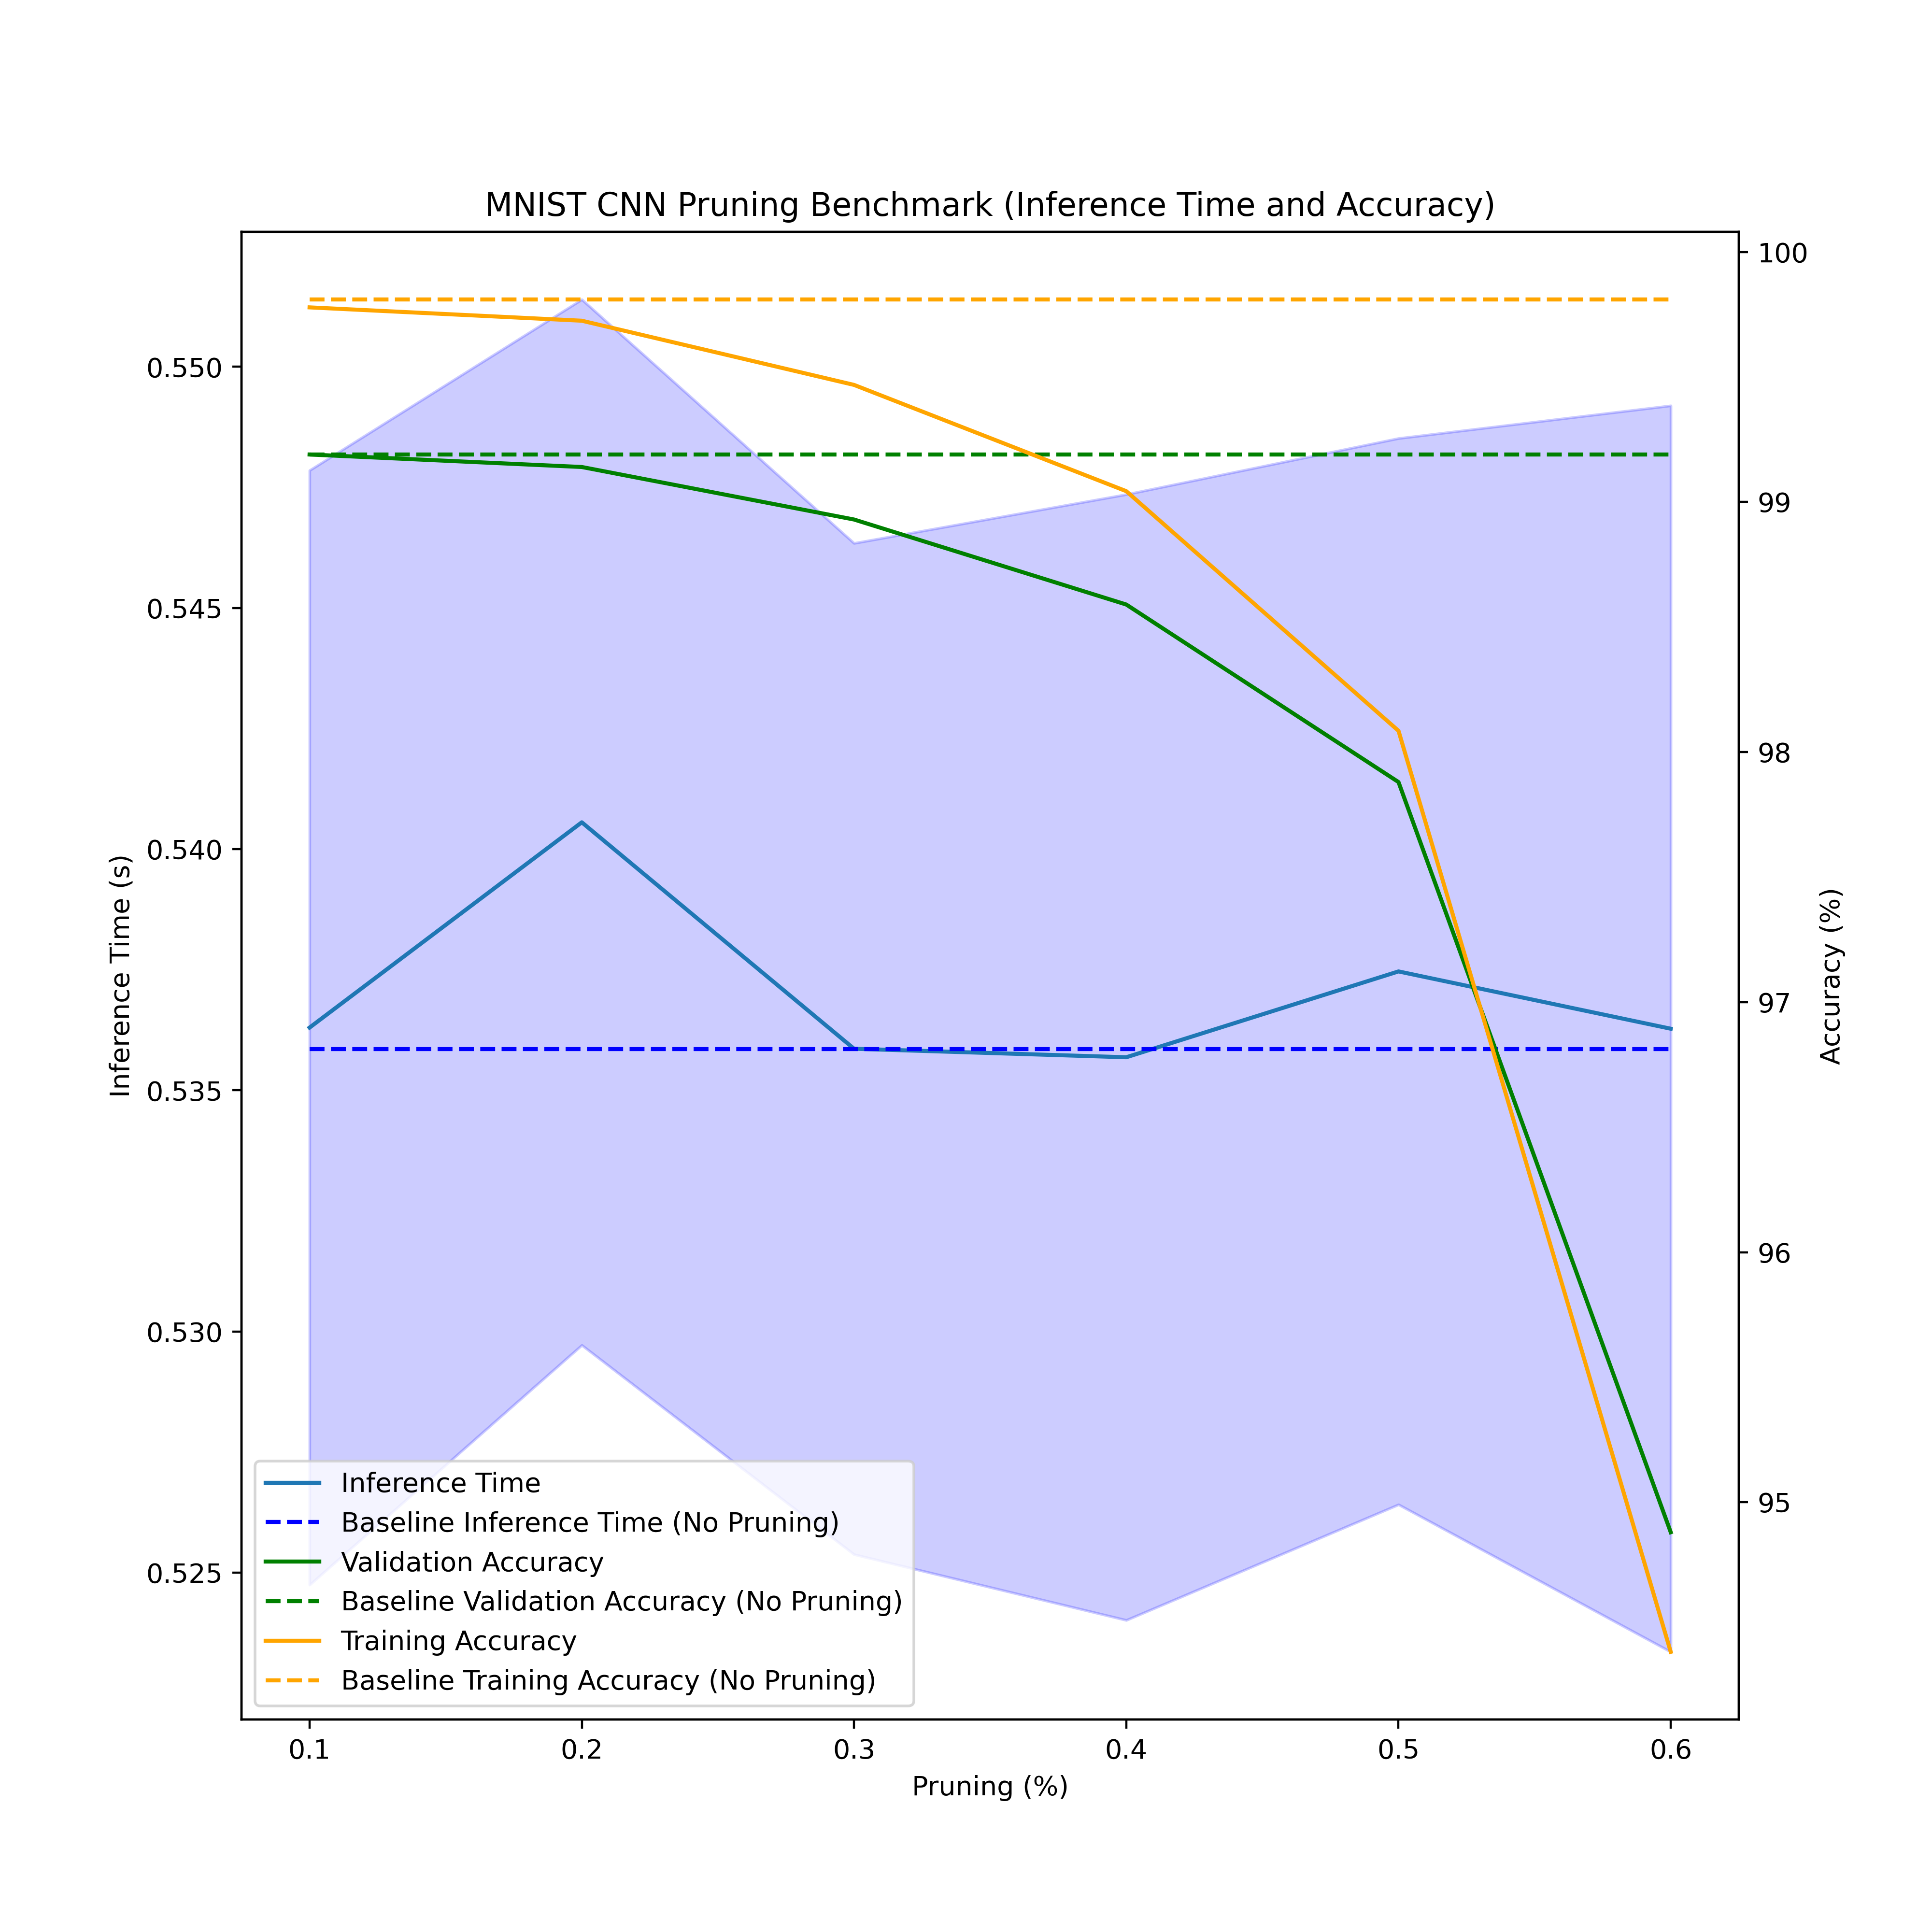
\includegraphics[width=4in]{../proj1/figures/mnist_cnn_benchmark.png}
		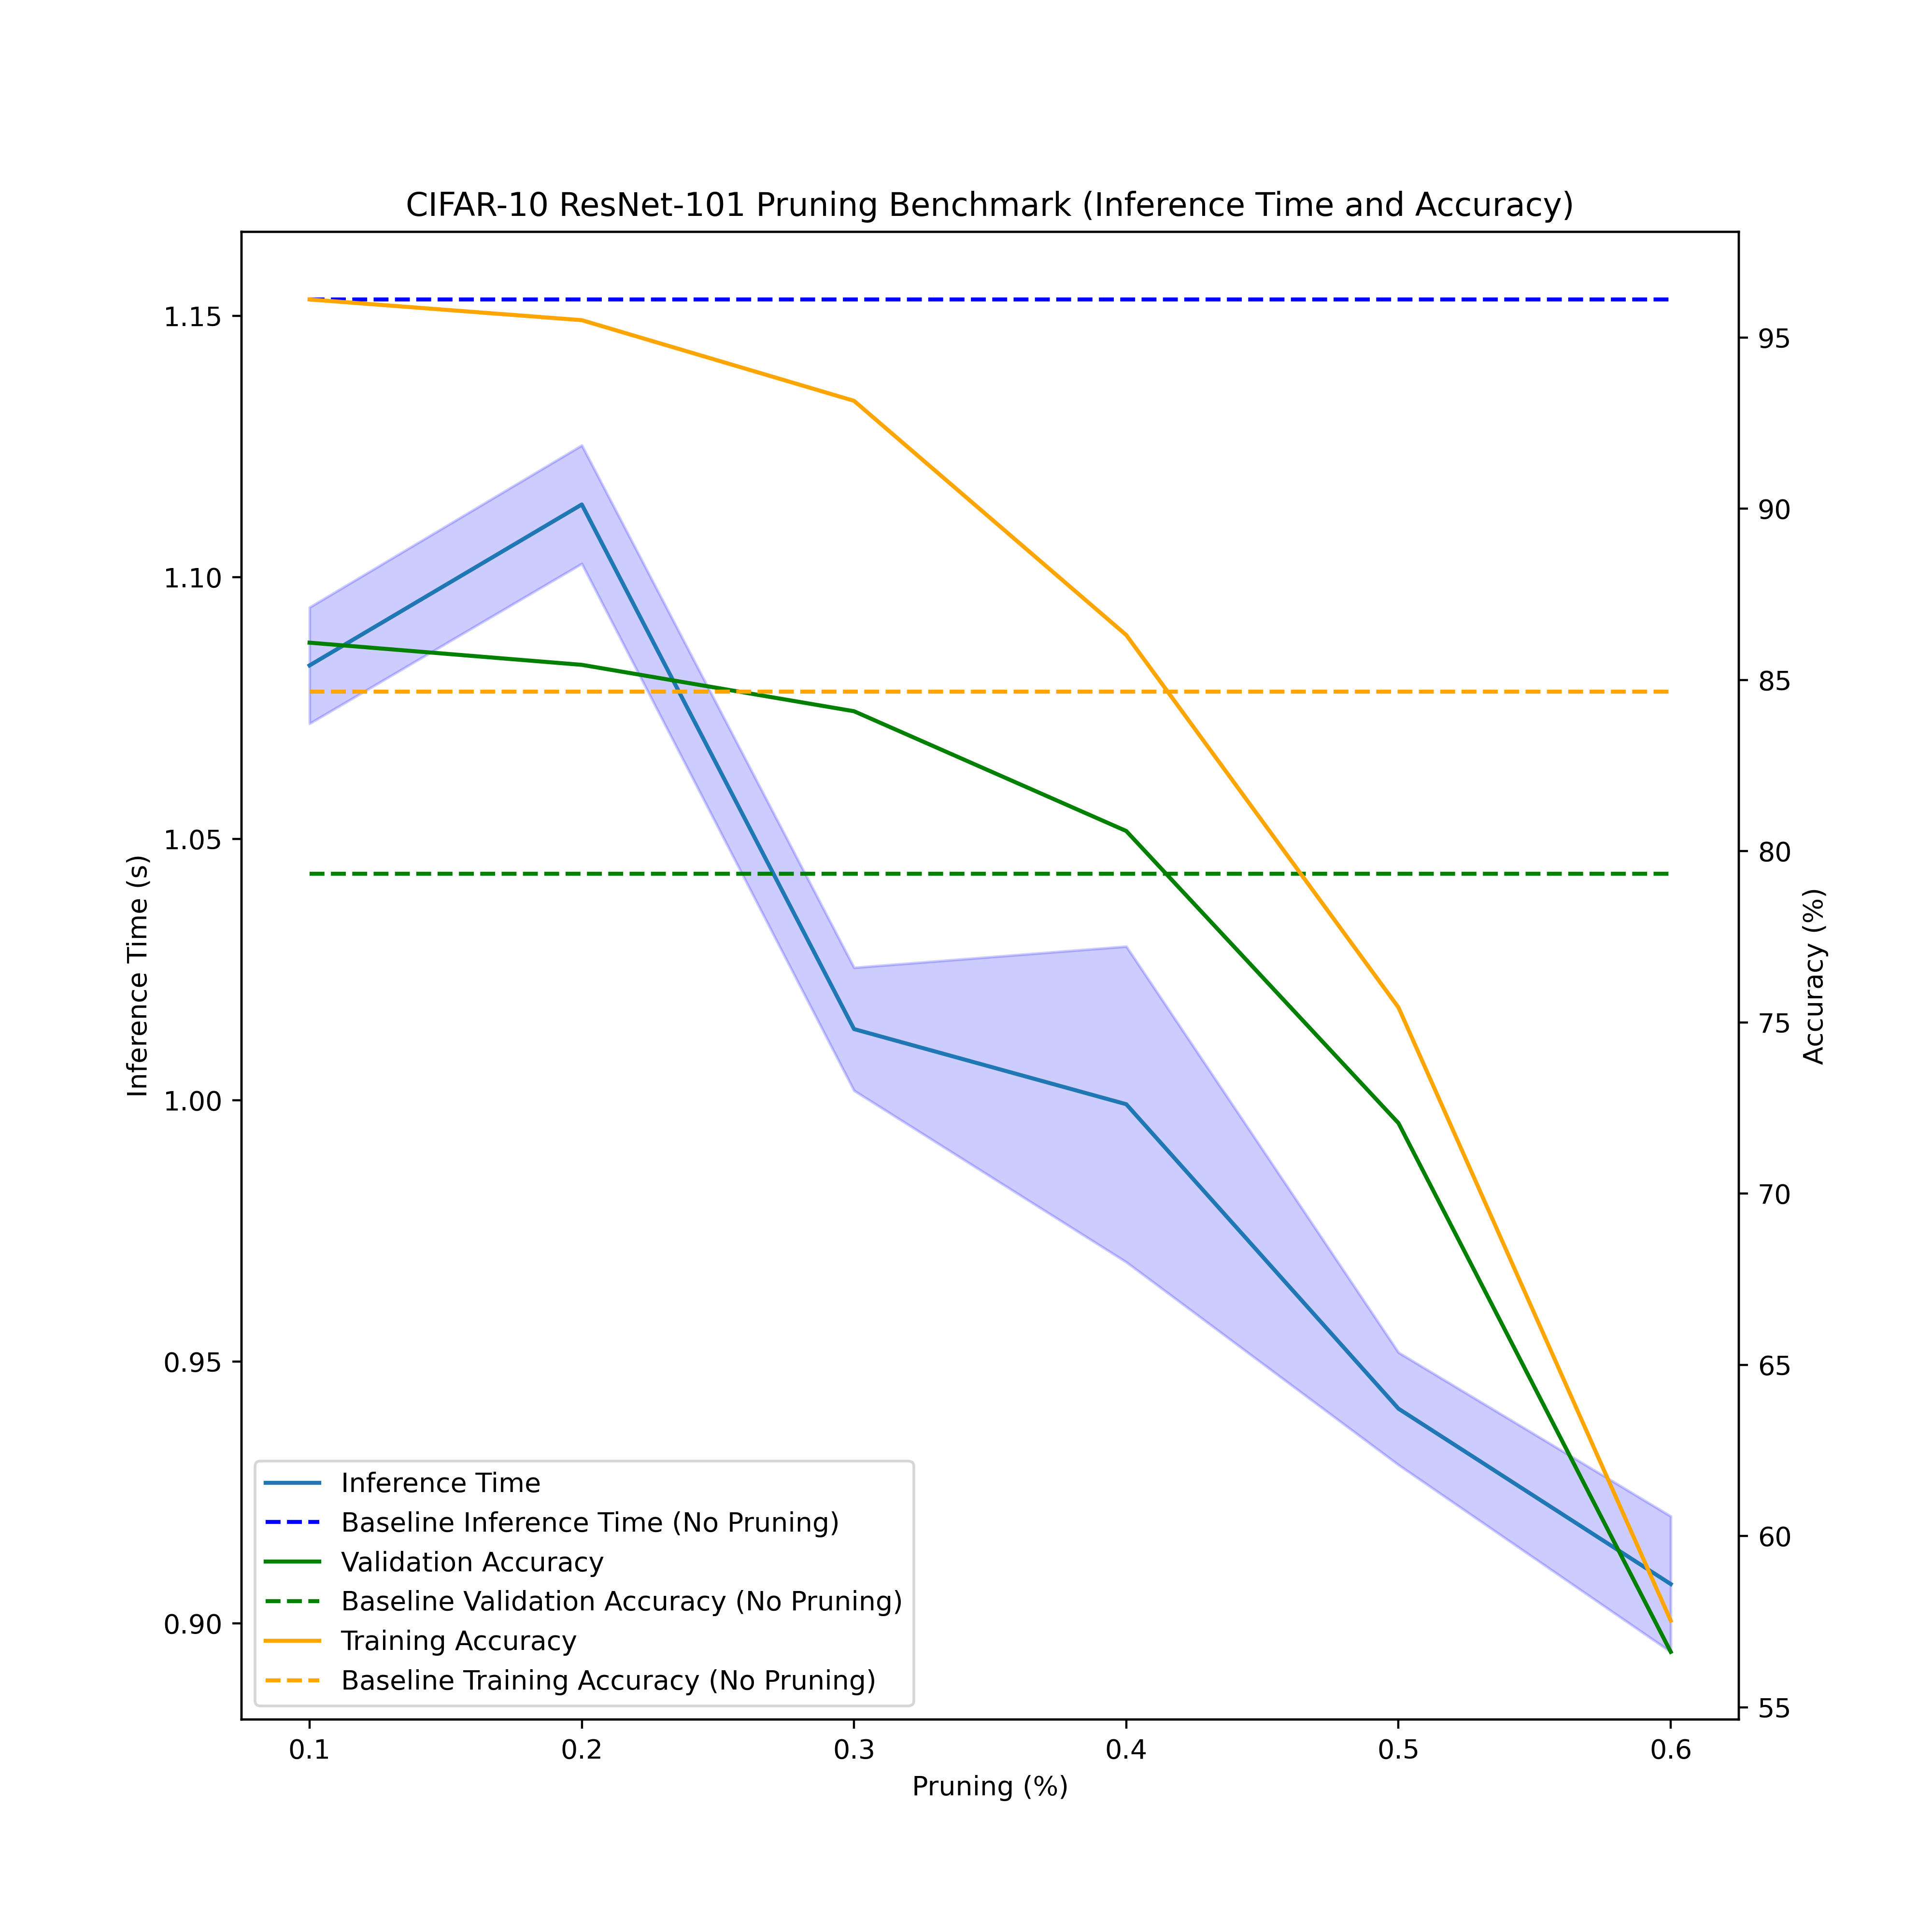
\includegraphics[width=4in]{../proj1/figures/resnet101_benchmark.png}
	}
	\caption{MNIST CNN and CIFAR 10 ResNet-101 Benchmark on NVIDIA A100}
	\label{fig:a100benchmark}
\end{figure}

The results are shown in Figure \ref{fig:a100benchmark} for NVIDIA A100 GPU. We report the inference time, training, and validation accuracy. We ran inference models for 25 trials and also plot the variance. We did this to see if there are any effects on cache misses on the GPU, as a higher variance across multiple trials may indicate it.

\begin{figure}
	\centerline{
		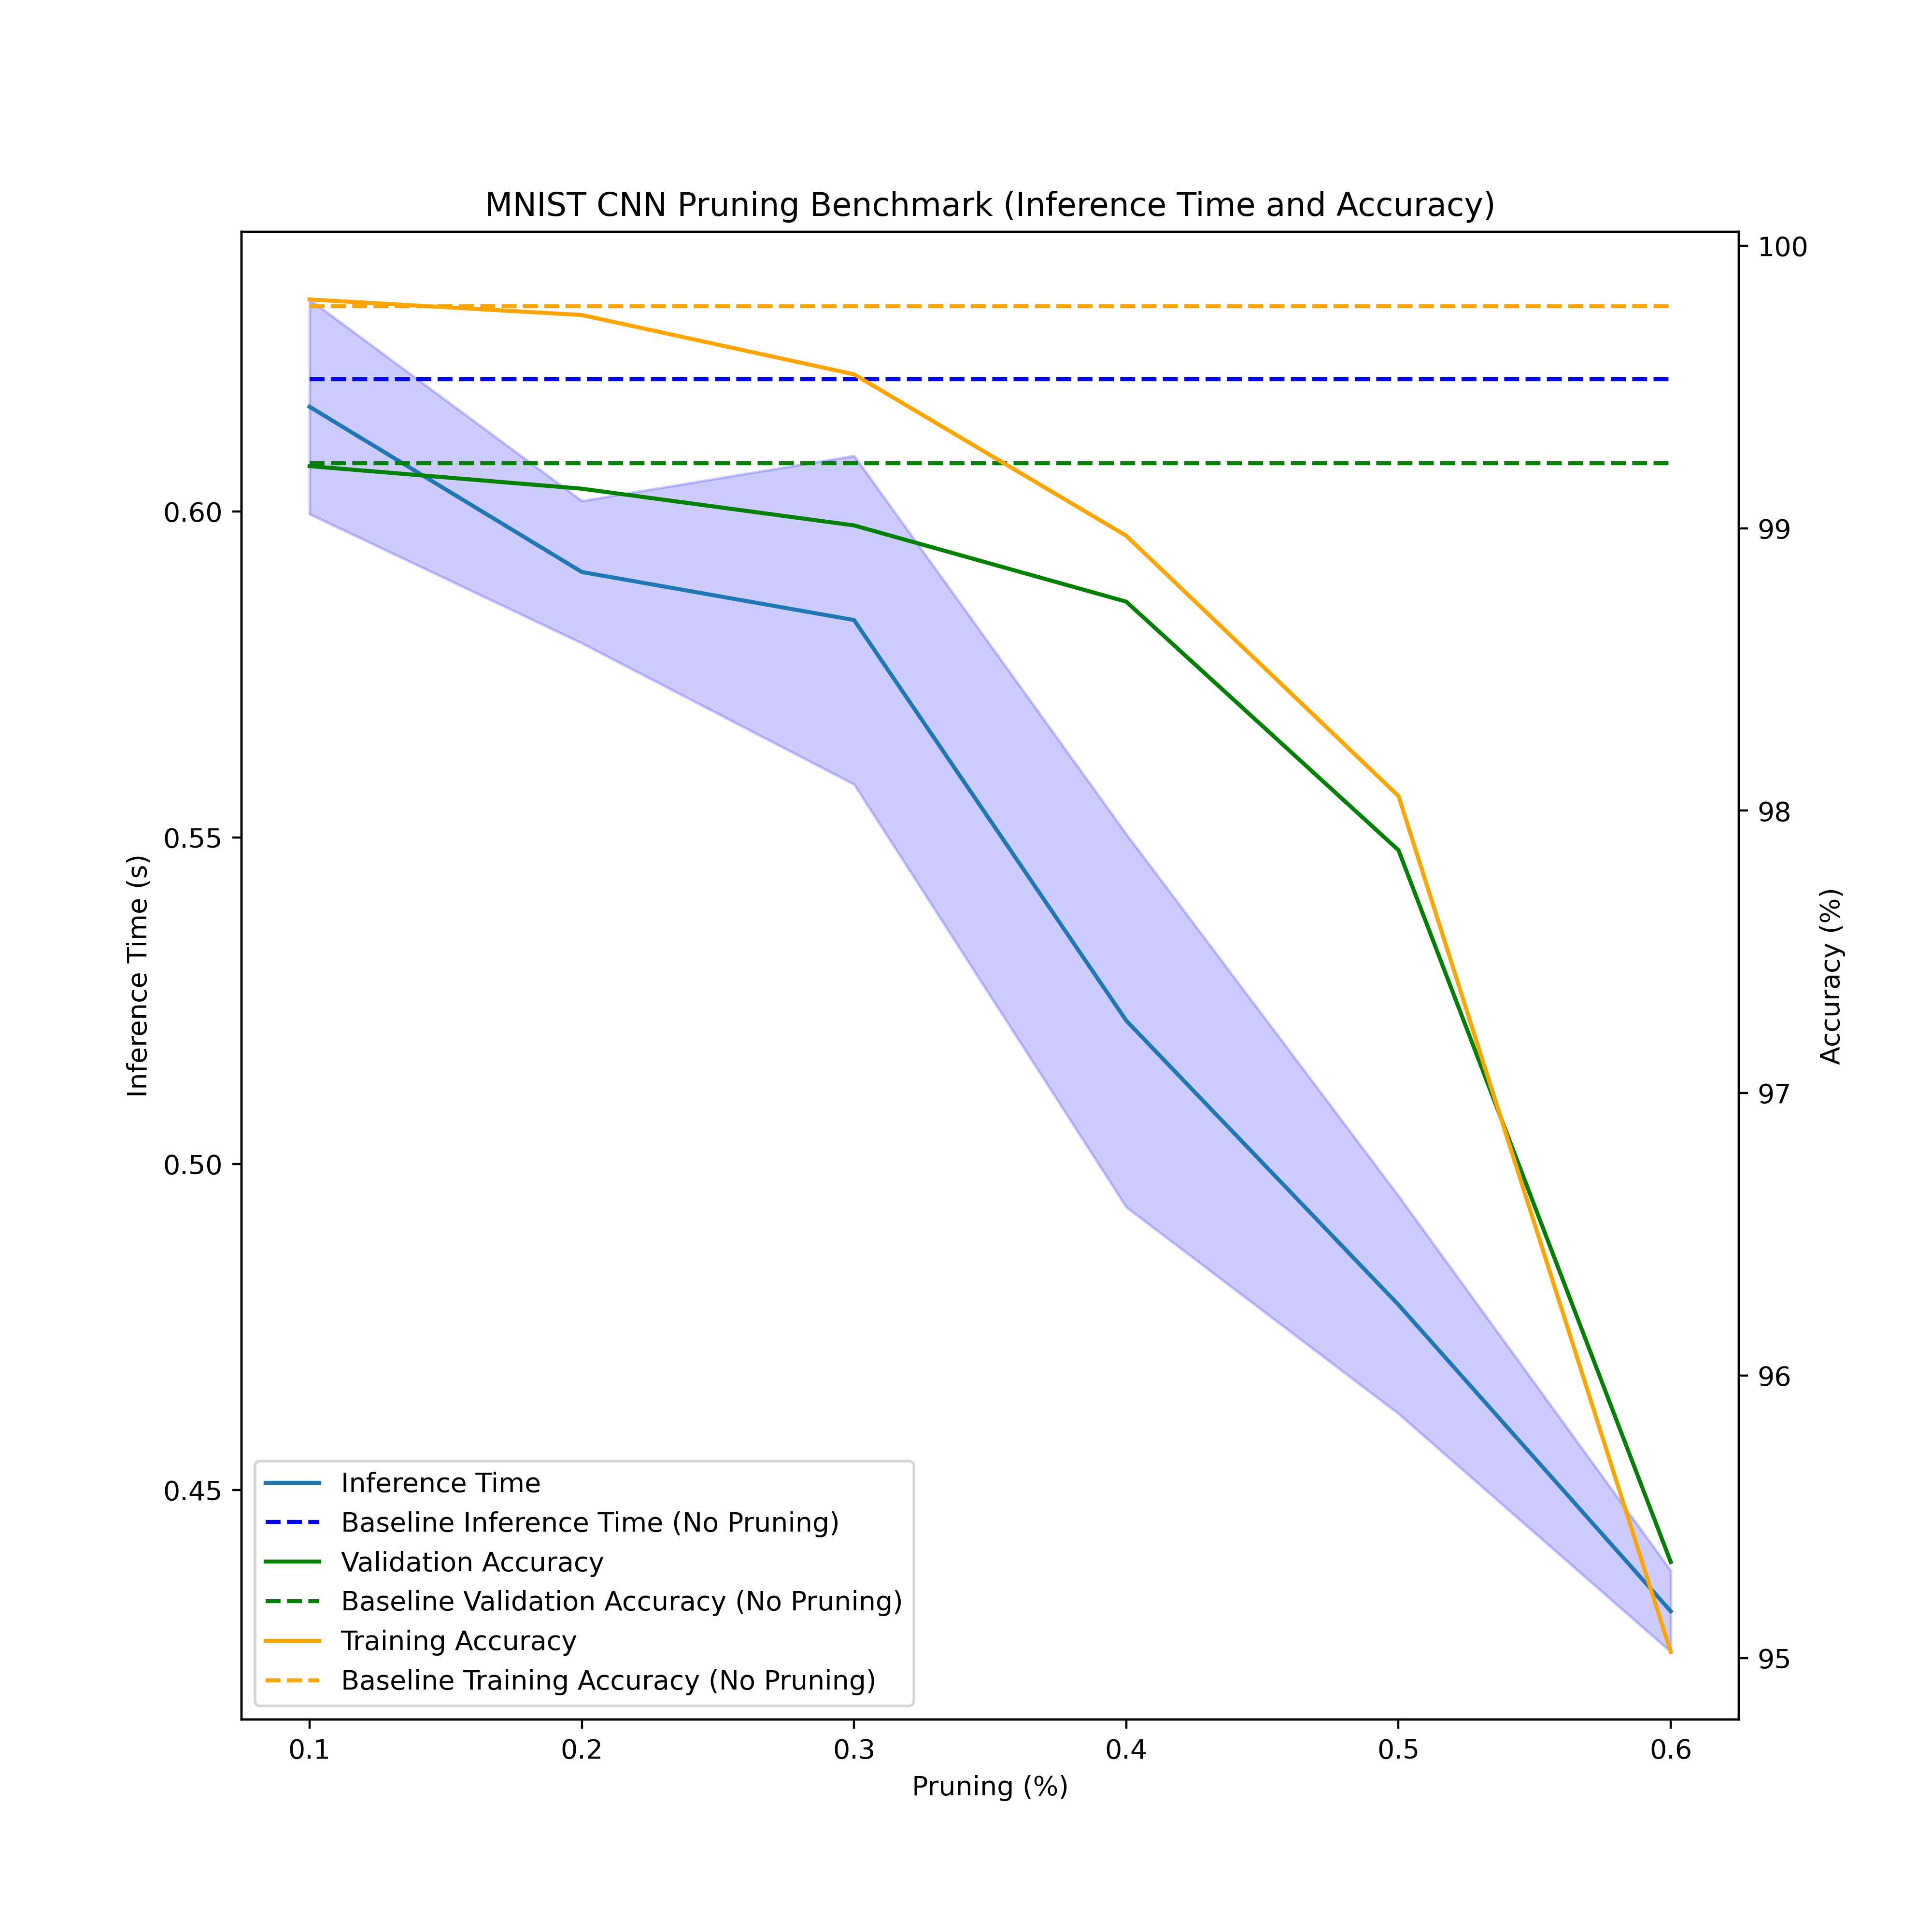
\includegraphics[width=4in]{../proj1/figures/mnist_cnn_benchmarkm1.png}
		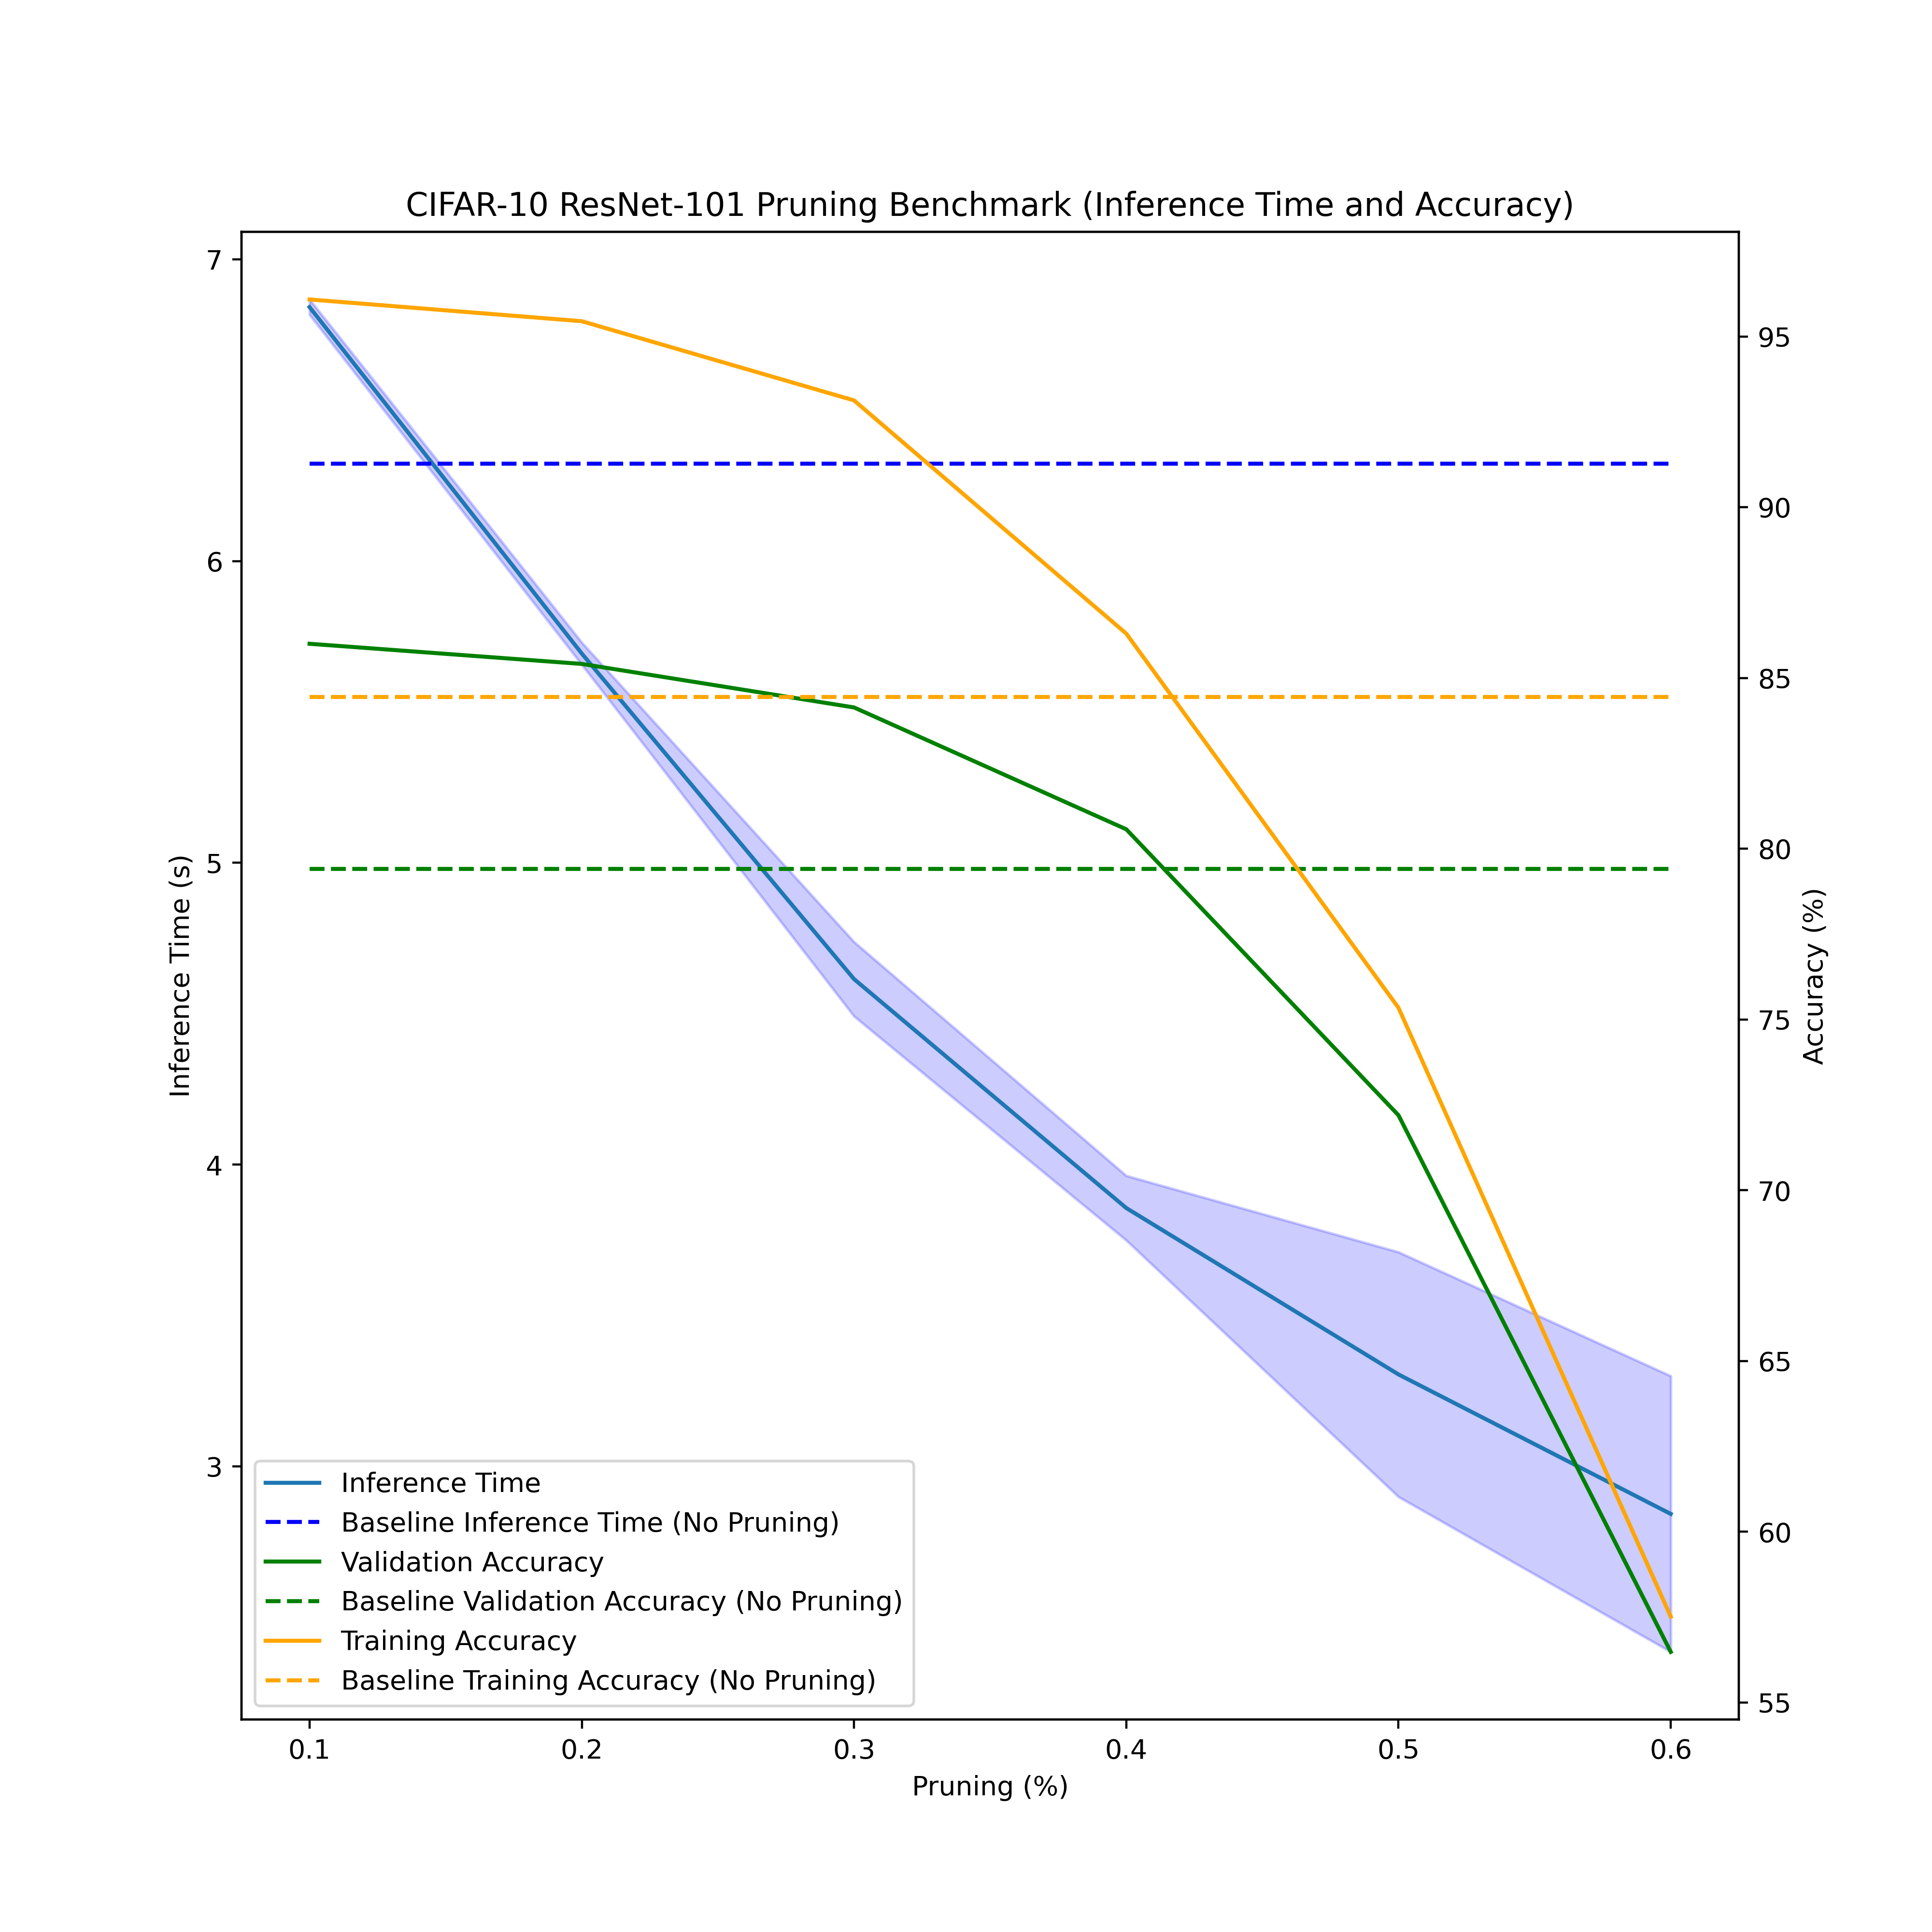
\includegraphics[width=4in]{../proj1/figures/resnet101_benchmarkm1.png}
	}
	\caption{MNIST CNN and CIFAR-10 ResNet-101 Benchmark on M1 MacBook Pro}
	\label{fig:m1benchmark}
\end{figure}

For M1 Mac, we're able to transfer the ResNet-101 weights from the node with the A100 we trained on. Then we ran just the inference models and got the results as reported in Figure \ref{fig:m1benchmark}. Another thing to keep in mind is that we don't see any synchronization primitives for the MPS kernels, and we're not exactly sure if the MPS GPU kernels are synchronous, or asynchronous like CUDA. The A100 inference time is also much more flat. We suspect that this might be due to overhead of memory transfer of the dataset from main memory to GPU HBM, making this memory bounded for such a small model. We don't see this effect in M1, as the memory between GPU and CPU is \textit{unified}, or shared.


For accuracy, the simple CNN degrades pretty quickly as the network becomes more sparse. This is what we expected to see. But interestingly the accuracy of ResNet-101 actually increases significantly. We're seeing training accuracy increase from 84\% to 96\% and validation accuracy increase from 79\% to 86\%. Both of the accuracies then start to degrade as the model becomes more sparse. The only suspicion is that retraining for 20 more epochs helped the model become more accurate. We also report our benchmarks for the \verb|L2NormPruner| and \verb|LevelPruner| in Figure \ref{fig:otherpruner}. The results are not comprehensive, as we didn't tune the configurations and parameters compared to \verb|L1NormPruner|. We wish to do more thorough analysis of why this happens, if time permits.

\begin{figure}
	\centerline{
		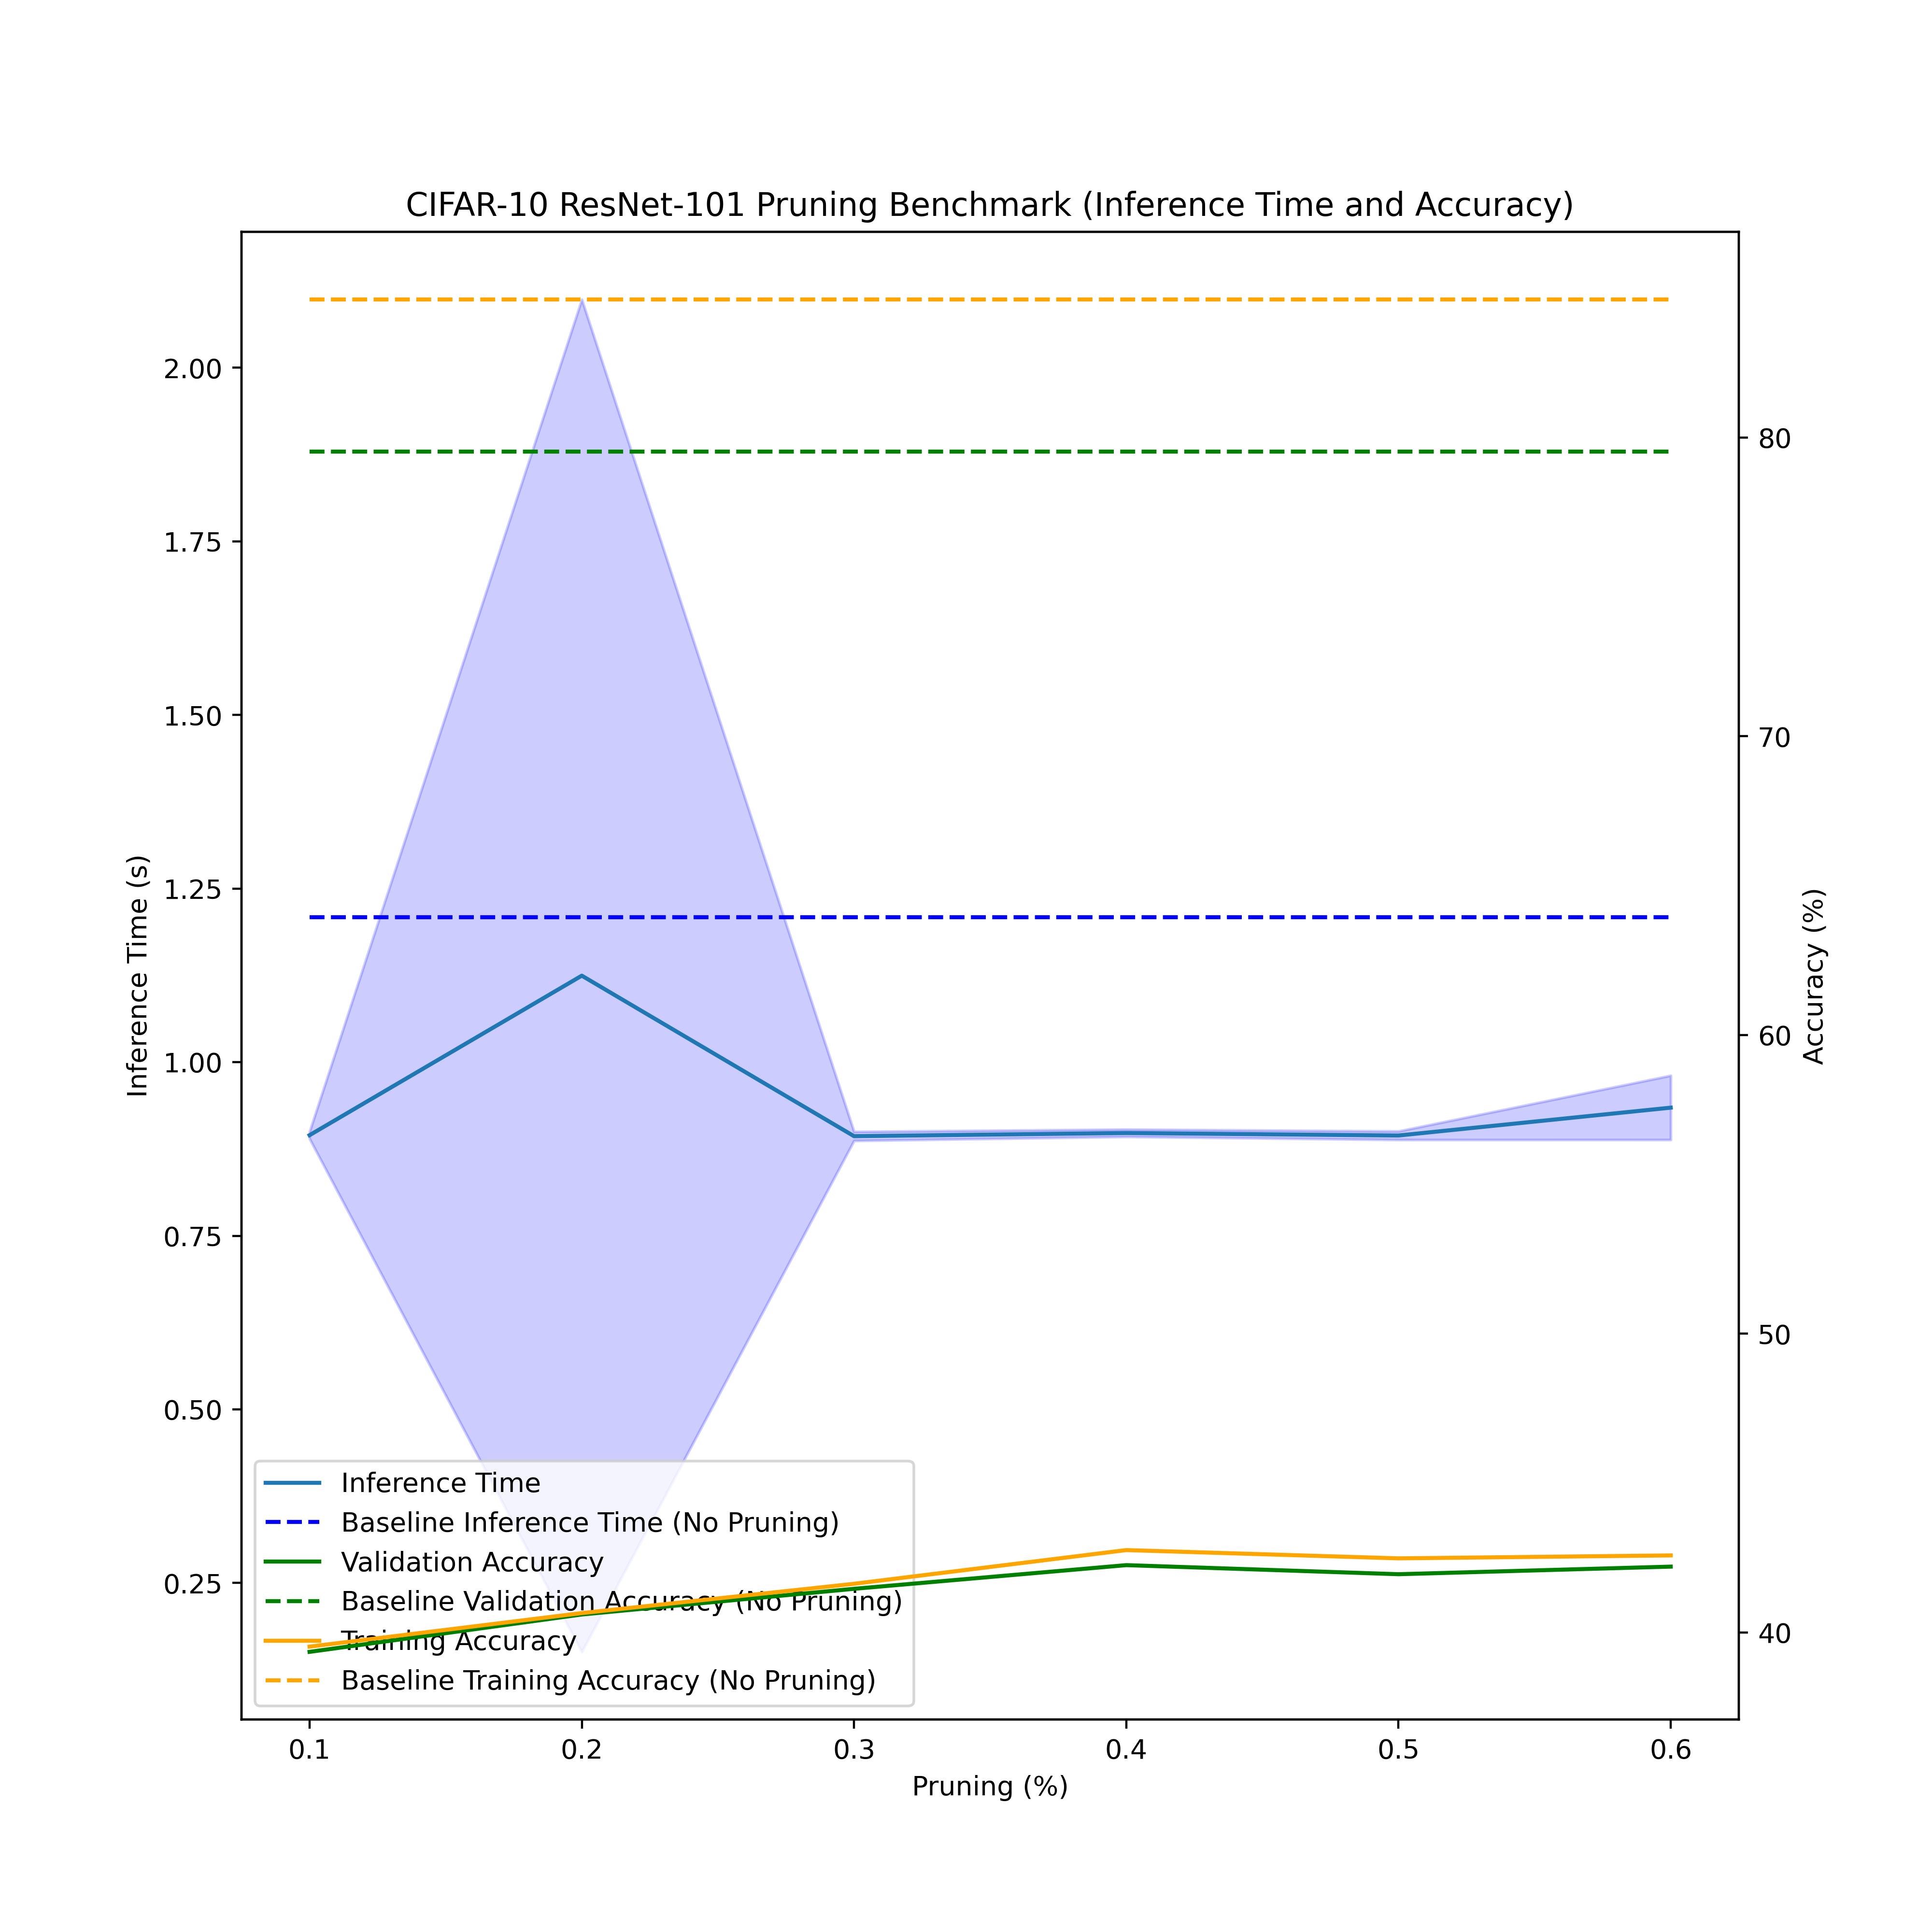
\includegraphics[width=4in]{../proj1/figures/resnet101_benchmark_l2.png}
		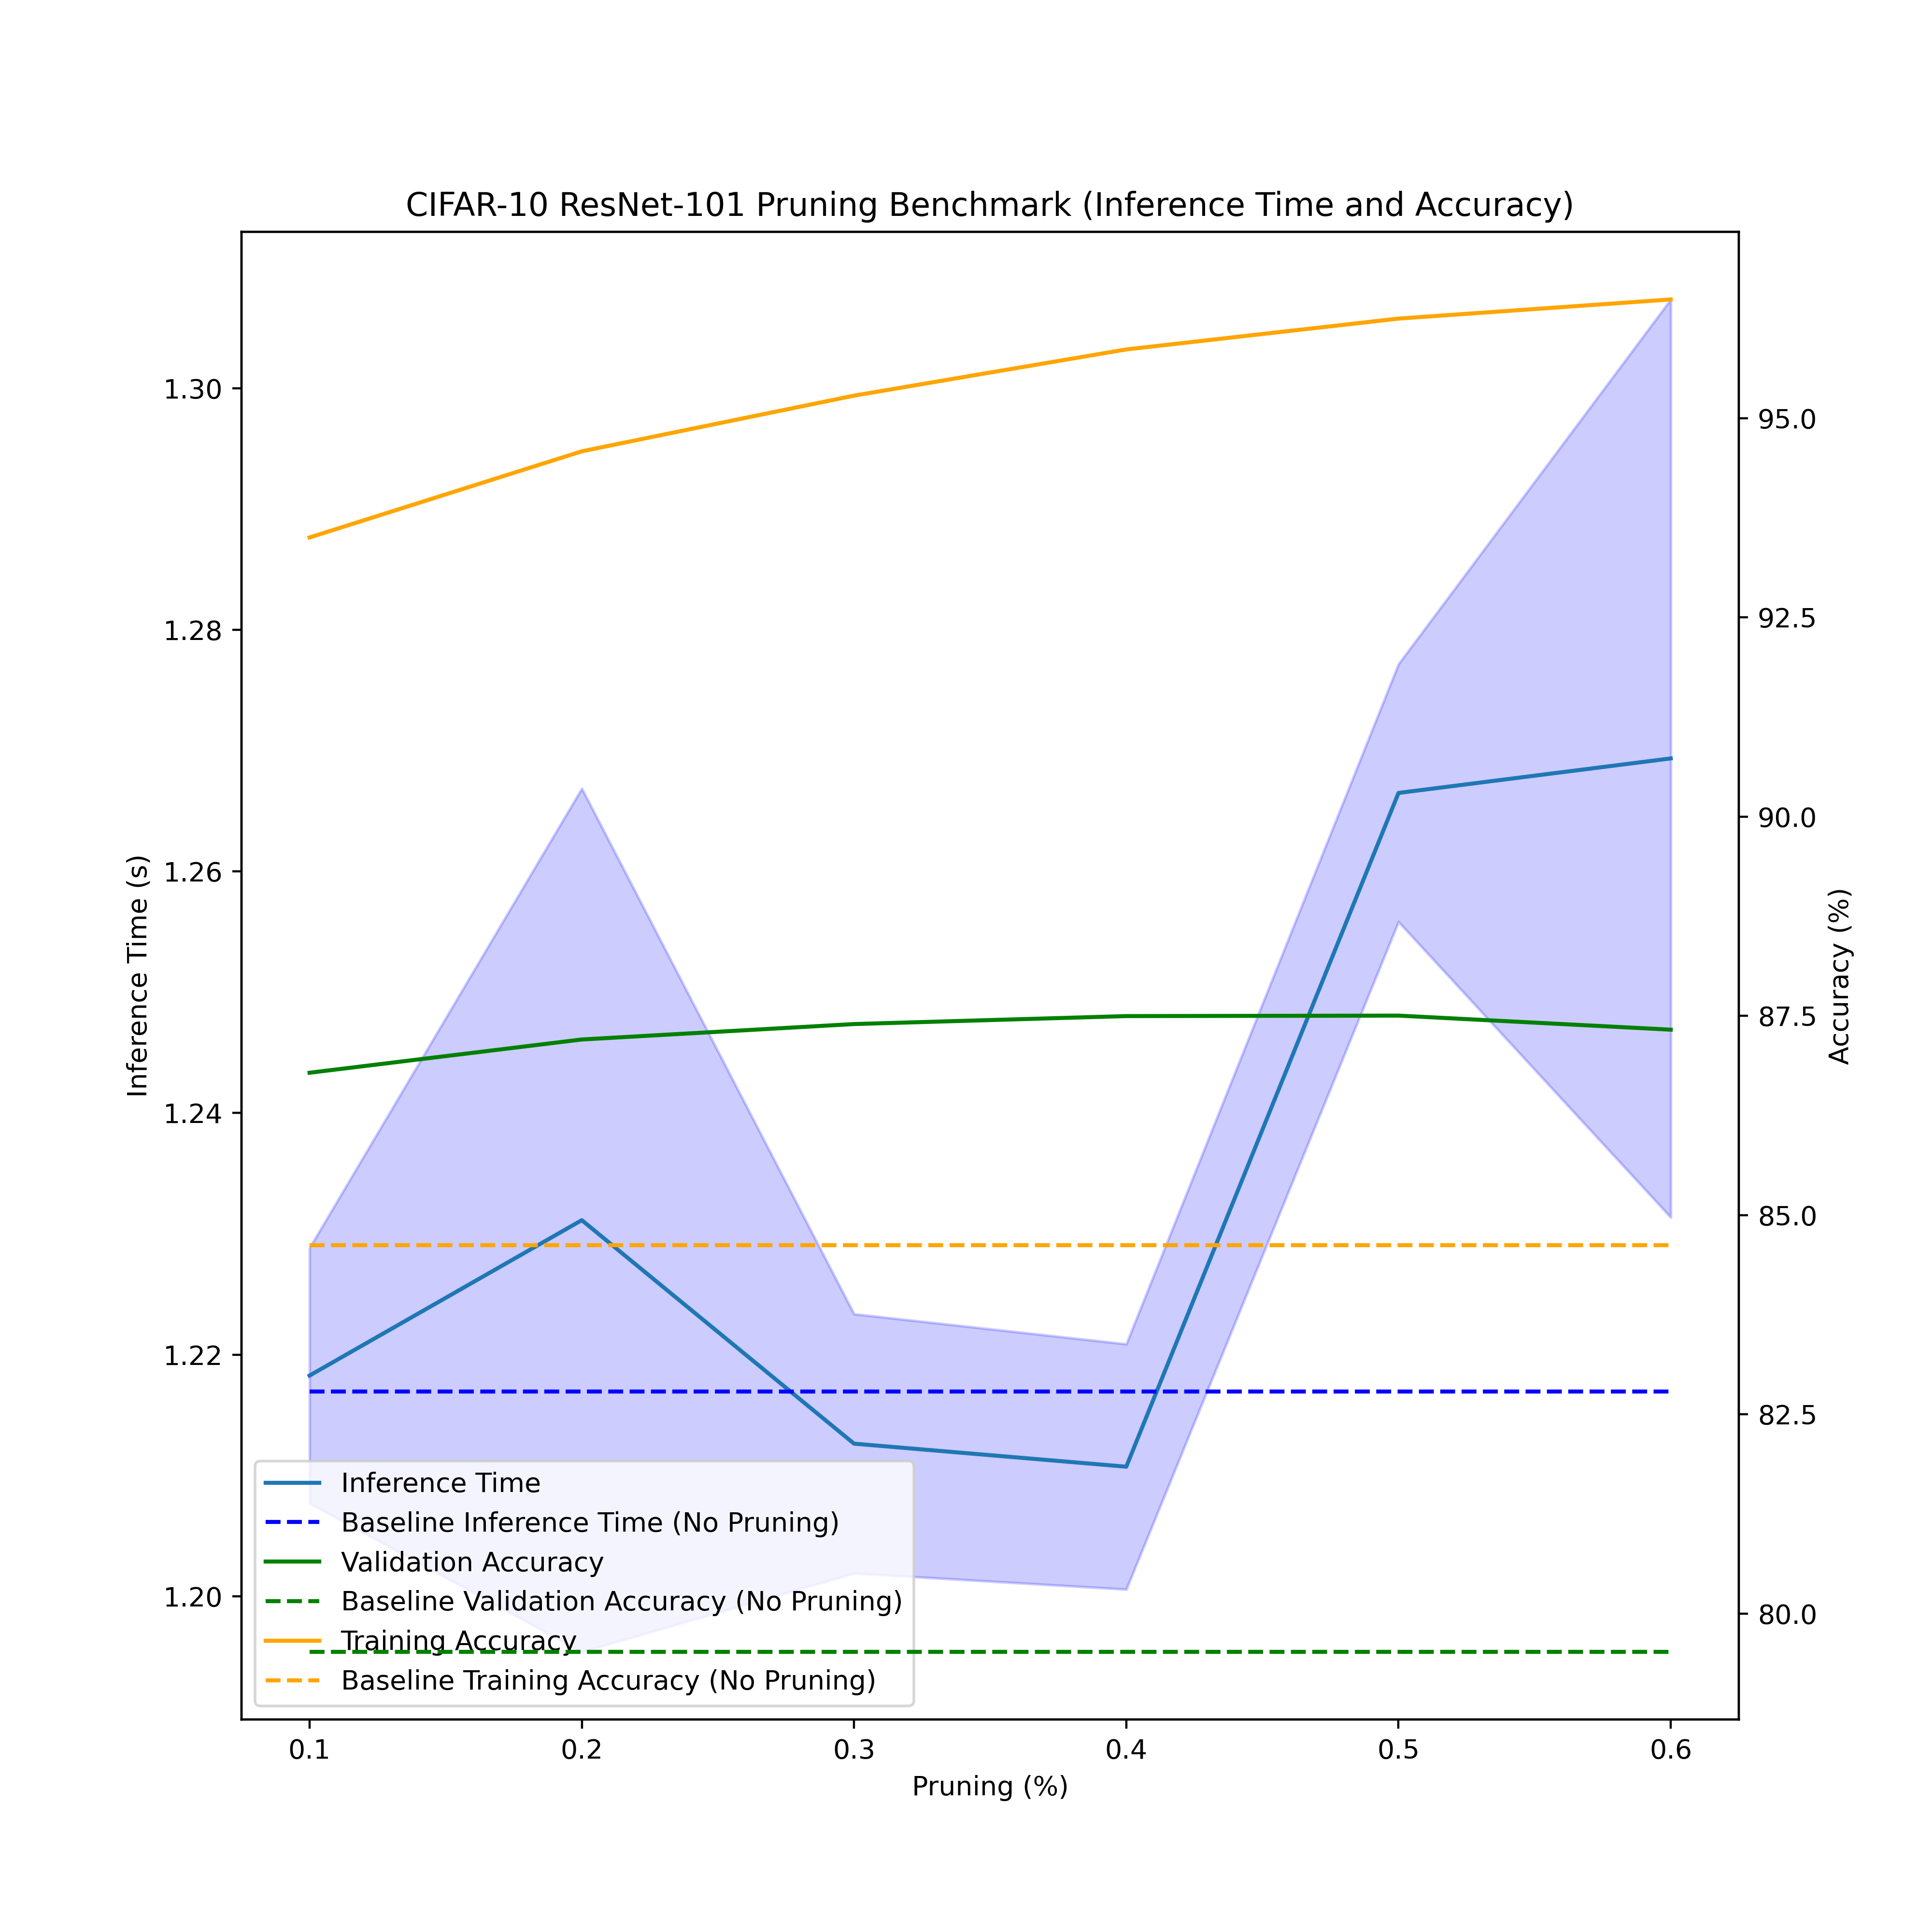
\includegraphics[width=4in]{../proj1/figures/resnet101_benchmark_level.png}
	}
	\caption{ResNet-101 Benchmark for L2NormPruner (left) and LevelPruner (right) on NVIDIA A100}
	\label{fig:otherpruner}
\end{figure}


\section{Lessons Learned}
%(4) What lessons you have learned through the project;
We learned how to use the PyTorch API at a much advanced level. Brian was a light PyTorch user, but he has learned how to utilize hardware acceleration via GPU on M1 Mac and CUDA to greatly speedup the training process for SOTA models, as well as other low level PyTorch functionalities.

We also learned that PyTorch also supports pruning, but only \textit{unstructured pruning}. With unstructured pruning, we would not achieve any speedups because it cannot exploit any parallelism. It turns out NNI is able to support structured pruning, thus why we are able to see noticeable speedups.

Although training was the main bottleneck to get things running, we also learned a lot from the effects of pruning. Pruning can have a great effect on inference speed. There's a certain sweetspot where we can achieve speedups until we degrade greatly in validation accuracy. It's also very mysterious how we can initially achieve higher accuracy after pruning. We cannot understand this phenomenon and wonder if our methodology is flawed somewhere, or whether it's actually true that pruning \textit{and} retraining can boost accuracy during the training process.

Lastly, it was our first time using PyTorch with a high end GPU and compare it against a mobile laptop GPU. We found the comparison of today's state of the hardware interesting from what is available in high performance clusters and consumer-end hardware.

\section{GitHub Repository}
The GitHub repository for this report is publicly accessible here \cite{repo}. To reproduce our findings, please read the \verb|README.md| under the \verb|proj1| directory. If there are any setup issues on ARC cluster, please contact \href{mailto:bcpark@ncsu.edu}{bcpark@ncsu.edu}.

\bibliographystyle{ieeetr}
\bibliography{references}

\section{Appendix}


\subsubsection{A1: Layers of Simple CNN for MNIST}
\label{sec:A1}
\begin{verbatim}
Net(
  (conv1): Conv2d(1, 16, kernel_size=(3, 3), stride=(1, 1))
  (conv2): Conv2d(16, 32, kernel_size=(3, 3), stride=(1, 1))
  (dropout1): Dropout(p=0.25, inplace=False)
  (dropout2): Dropout(p=0.5, inplace=False)
  (fc1): Linear(in_features=4608, out_features=64, bias=True)
  (fc2): Linear(in_features=64, out_features=10, bias=True)
)
\end{verbatim}
With 60\% Pruning ratio:
\begin{verbatim}
Net(
  (conv1): Conv2d(1, 3, kernel_size=(3, 3), stride=(1, 1))
  (conv2): Conv2d(3, 4, kernel_size=(3, 3), stride=(1, 1))
  (dropout1): Dropout(p=0.25, inplace=False)
  (dropout2): Dropout(p=0.5, inplace=False)
  (fc1): Linear(in_features=576, out_features=8, bias=True)
  (fc2): Linear(in_features=8, out_features=10, bias=True)
)
\end{verbatim}


\subsubsection{A2: Layers of ResNet18 for CIFAR-10}
\label{sec:A2}
\begin{verbatim}
ResNet(
  (conv1): Conv2d(3, 64, kernel_size=(7, 7), stride=(2, 2), padding=(3, 3), bias=False)
  (bn1): BatchNorm2d(64, eps=1e-05, momentum=0.1, affine=True, track_running_stats=True)
  (relu): ReLU(inplace=True)
  (maxpool): MaxPool2d(kernel_size=3, stride=2, padding=1, dilation=1, ceil_mode=False)
  (layer1): Sequential(
    (0): BasicBlock(
      (conv1): Conv2d(64, 64, kernel_size=(3, 3), stride=(1, 1), padding=(1, 1), bias=False)
      (bn1): BatchNorm2d(64, eps=1e-05, momentum=0.1, affine=True, track_running_stats=True)
      (relu): ReLU(inplace=True)
      (conv2): Conv2d(64, 64, kernel_size=(3, 3), stride=(1, 1), padding=(1, 1), bias=False)
      (bn2): BatchNorm2d(64, eps=1e-05, momentum=0.1, affine=True, track_running_stats=True)
    )
    (1): BasicBlock(
      (conv1): Conv2d(64, 64, kernel_size=(3, 3), stride=(1, 1), padding=(1, 1), bias=False)
      (bn1): BatchNorm2d(64, eps=1e-05, momentum=0.1, affine=True, track_running_stats=True)
      (relu): ReLU(inplace=True)
      (conv2): Conv2d(64, 64, kernel_size=(3, 3), stride=(1, 1), padding=(1, 1), bias=False)
      (bn2): BatchNorm2d(64, eps=1e-05, momentum=0.1, affine=True, track_running_stats=True)
    )
  )
  (layer2): Sequential(
    (0): BasicBlock(
      (conv1): Conv2d(64, 128, kernel_size=(3, 3), stride=(2, 2), padding=(1, 1), bias=False)
      (bn1): BatchNorm2d(128, eps=1e-05, momentum=0.1, affine=True, track_running_stats=True)
      (relu): ReLU(inplace=True)
      (conv2): Conv2d(128, 128, kernel_size=(3, 3), stride=(1, 1), padding=(1, 1), bias=False)
      (bn2): BatchNorm2d(128, eps=1e-05, momentum=0.1, affine=True, track_running_stats=True)
      (downsample): Sequential(
        (0): Conv2d(64, 128, kernel_size=(1, 1), stride=(2, 2), bias=False)
        (1): BatchNorm2d(128, eps=1e-05, momentum=0.1, affine=True, track_running_stats=True)
      )
    )
    (1): BasicBlock(
      (conv1): Conv2d(128, 128, kernel_size=(3, 3), stride=(1, 1), padding=(1, 1), bias=False)
      (bn1): BatchNorm2d(128, eps=1e-05, momentum=0.1, affine=True, track_running_stats=True)
      (relu): ReLU(inplace=True)
      (conv2): Conv2d(128, 128, kernel_size=(3, 3), stride=(1, 1), padding=(1, 1), bias=False)
      (bn2): BatchNorm2d(128, eps=1e-05, momentum=0.1, affine=True, track_running_stats=True)
    )
  )
  (layer3): Sequential(
    (0): BasicBlock(
      (conv1): Conv2d(128, 256, kernel_size=(3, 3), stride=(2, 2), padding=(1, 1), bias=False)
      (bn1): BatchNorm2d(256, eps=1e-05, momentum=0.1, affine=True, track_running_stats=True)
      (relu): ReLU(inplace=True)
      (conv2): Conv2d(256, 256, kernel_size=(3, 3), stride=(1, 1), padding=(1, 1), bias=False)
      (bn2): BatchNorm2d(256, eps=1e-05, momentum=0.1, affine=True, track_running_stats=True)
      (downsample): Sequential(
        (0): Conv2d(128, 256, kernel_size=(1, 1), stride=(2, 2), bias=False)
        (1): BatchNorm2d(256, eps=1e-05, momentum=0.1, affine=True, track_running_stats=True)
      )
    )
    (1): BasicBlock(
      (conv1): Conv2d(256, 256, kernel_size=(3, 3), stride=(1, 1), padding=(1, 1), bias=False)
      (bn1): BatchNorm2d(256, eps=1e-05, momentum=0.1, affine=True, track_running_stats=True)
      (relu): ReLU(inplace=True)
      (conv2): Conv2d(256, 256, kernel_size=(3, 3), stride=(1, 1), padding=(1, 1), bias=False)
      (bn2): BatchNorm2d(256, eps=1e-05, momentum=0.1, affine=True, track_running_stats=True)
    )
  )
  (layer4): Sequential(
    (0): BasicBlock(
      (conv1): Conv2d(256, 512, kernel_size=(3, 3), stride=(2, 2), padding=(1, 1), bias=False)
      (bn1): BatchNorm2d(512, eps=1e-05, momentum=0.1, affine=True, track_running_stats=True)
      (relu): ReLU(inplace=True)
      (conv2): Conv2d(512, 512, kernel_size=(3, 3), stride=(1, 1), padding=(1, 1), bias=False)
      (bn2): BatchNorm2d(512, eps=1e-05, momentum=0.1, affine=True, track_running_stats=True)
      (downsample): Sequential(
        (0): Conv2d(256, 512, kernel_size=(1, 1), stride=(2, 2), bias=False)
        (1): BatchNorm2d(512, eps=1e-05, momentum=0.1, affine=True, track_running_stats=True)
      )
    )
    (1): BasicBlock(
      (conv1): Conv2d(512, 512, kernel_size=(3, 3), stride=(1, 1), padding=(1, 1), bias=False)
      (bn1): BatchNorm2d(512, eps=1e-05, momentum=0.1, affine=True, track_running_stats=True)
      (relu): ReLU(inplace=True)
      (conv2): Conv2d(512, 512, kernel_size=(3, 3), stride=(1, 1), padding=(1, 1), bias=False)
      (bn2): BatchNorm2d(512, eps=1e-05, momentum=0.1, affine=True, track_running_stats=True)
    )
  )
  (avgpool): AdaptiveAvgPool2d(output_size=(1, 1))
  (fc): Linear(in_features=512, out_features=1000, bias=True)
)
\end{verbatim}
\end{document}